\documentclass{ctexart}
\usepackage{ctex}
\usepackage{graphicx}
\usepackage{amsmath}
\usepackage{amsfonts}


\graphicspath{{figures/}}  %指定图片路径

\title{不同近邻数的高效$ KNN $分类}
\author{Mr Wu}
\date{\today}

\begin{document}
	\maketitle
	\section{摘要}
	传统KNN算法为所有测试样本赋予相同$ k $值,不切实际。之前的解决方法通过交叉验证来为不同的样本赋不同的$ k $值,但是通常比较耗时。本文提出了一个$ kTree $的方法,通过在$ KNN $分类过程中加入一个训练阶段,来为不同的样本学习不同的最佳$ k $值。
	
	在训练阶段,$ kTree $方法首先通过一个新的稀疏重构模型为所有样本学习最佳$ k $值,然后用训练样本和得到的最佳$ k $值构建决策树,也就是$ kTree $。在测试阶段,$ kTree $为每个测试样本快速输出最佳$ k $值,学习到的$ k $值和所有训练样本可以用来指导$ KNN $分类。与传统方法相比,此方法运行代价相当,但准确率更高。与新的为不同样本赋予不同$ k $值的算法相比,分类准确率相似,但运行代价更低。
	
	这篇文章还提出了$ kTree $方法的一个改进版本,通过将训练样本的信息存储在叶节点来加速测试阶段。
	\section{介绍}
	Sahigara提出应用蒙特卡洛交叉验证来为每个测试样本选取一个最佳的光滑参数k。Zhang基于一个重构框架来学习k值。
	
	不管是学习k值的过程,还是寻找最近邻的过程,都很耗时。因此同时解决这些问题很有挑战性,也就是:为不同样本学习最佳k值,降低时间复杂度,提升表现。
	
	本文中,在训练阶段,首先利用所有样本,通过设计一个基于稀疏的重构模型,来重构所有训练样本,于是能为每个训练样本输出一个最佳k值。然后用训练样本和它们对应的最佳k值构建一个决策树,也就是将学习到的最佳k值作为每个样本的标签。训练阶段是离线的,每个叶节点存储一个最佳k值。在测试阶段,首先在kTree中从根结点搜索到一个叶子结点,将其中的k值赋给这个测试样本。然后用传统KNN算法,用多数表决原则为其分类。
	
	我们的方法和其它方法有两个显著区别。一是之前的方法没有训练阶段,我们的方法有一个基于稀疏的训练阶段,时间复杂度为$ O(n^2) $。二是之前的方法学习到最佳k值需要$ O(n^2) $的复杂度,我们的算法只需要$ O(log(d)+n) $(其中d是特征维数)。
	
	尽管我们的kTree方法能得到所有测试样本的最佳k值,但仍然需要扫描所有训练样本来执行kNN分类,这是一个耗时的过程,最少需要$ O(n^2d) $。于是我们将kTree方法改进为k*Tree方法,通过将训练样本的额外信息存储在剩余节点(比如训练样本的最近邻,以及最近邻的最近邻)来加速测试阶段。将得到的决策树称为k*Tree。
	
	\section{相关工作}
	kNN方法的性能被很多因素影响,如k值选取,距离的度量。为了解决这些问题,很多机器学习技巧被提出。
	很多方法解决了选取不同k值的问题,但是它们的复杂度很高。
	
	\section{方法} %\mathbb空心粗体,用amsfonts宏包;\boldsymbol{X}:斜黑体;$\mathbf{text}$:直立黑体
	\subsection{重构}
	训练样本$ \mathbf{X} \in \mathbb{R}^{d \times n} = [\mathbf{x_1}, ..., \mathbf{x_n}]$, $ n $ 和$ d $表示训练样本的数量和维度。我们用训练样本来重构自身,目标是最小化$ \mathbf{Xw_i} \text{与} \mathbf{x_i} $ 的距离(其中$ \mathbf{w_i} $是重构系数矩阵)。用如下的最小二乘损失函数:
	\begin{equation}
		\min_\mathbf{W} \sum_{i=1}^{n} \Arrowvert{\mathbf{Xw_i} - \mathbf{x_i}} \Arrowvert_{2}^{2} = \min_\mathbf{W} \Arrowvert{\mathbf{XW-X}}\Arrowvert_F^2
	\end{equation}
	其中$ \mathbf{W} $是重构系数矩阵,表示训练样本之间的关系。
	
	实际应用中,为了避免$ \mathbf{X^TX} $是奇异矩阵所带来的问题,通常加上一个$ l_2 $范数的正则项:
	\begin{equation}
		\min_\mathbf{W} \Arrowvert{\mathbf{XW-X}}\Arrowvert_{F}^{2} + \rho \Arrowvert{\mathbf W}\Arrowvert_2^2	
	\end{equation}
	上式称为岭回归,有闭式解$ \mathbf W = (\mathbf{X^TX} + \rho\mathbf I)^{-1}  \mathbf{X^TX}$。然而(2)式不能产生稀疏结果。在这篇文章里,我们想产生稀疏的重构系数,从而只选择训练样本的一部分来重构每个测试样本。于是参考之前的文献,有如下的稀疏目标函数:
	\begin{equation}
	\min_\mathbf{W} \Arrowvert{\mathbf{XW-X}}\Arrowvert_{F}^{2} + \rho_1 \Arrowvert{\mathbf W}\Arrowvert_1,\mathbf W \succeq 0
	\end{equation}
	其中$ \mathbf W \succeq 0  $表示$ \mathbf W $ 的每个元素非负。(3)式已被证明能产生稀疏的$ \mathbf W $。$ 且\rho_1 $的值越大,$ \mathbf W $越稀疏。
	
	我们用训练样本来重构自身,就期望在样本或特征之间存在关联。一般来说,如果两个特征高度相关,它们的预测也是相关的。我们通过定义如下函数,将$ \mathbf{X} $中两个训练样本的关联映射到它们的预测中:
	\begin{equation}
	\frac{1}{2}\sum_{i,j}^{d}s_{ij}\Arrowvert{\mathbf{x^iW-x^jW}}\Arrowvert_2^2
	\end{equation}
	$ S $是相似度矩阵,至于向量间的相似度定义,我们用一个如下定义的径向基核函数:
	\begin{equation}
		f(\mathbf{a,b}) = exp(-\frac{\Arrowvert \mathbf{a-b} \Arrowvert_2^2}{2\sigma^2}) \label{eq:kernel}
	\end{equation}
	其中$\sigma$表示核宽度。至于相似度矩阵$ S $,首先通过将每个特征看做一个结点,并用$ kNN $以及(\ref{eq:kernel})中定义的核函数,来构建一个数据邻接图。例如:特征$ x^j $被选为特征$ x^i $的$ k $近邻之一,则$ s_{ij} = f(\mathbf{x^i, x^j}) $。否则,相似度设为0。
	
	经过简单的数学变换,得到如下正则项:
	\begin{equation}
		\mathbf{R(W)} = \mathbf{Tr(W^TX^TLXW)}
	\end{equation}
	其中$ \mathbf L \in \mathbb{R}^{d \times d} $是拉普拉斯矩阵。要注意这里$ \mathbf L $的定义与文献[43]和[58]不一样,这里的拉普拉斯矩阵表明的是特征之间的关联信息。最终得到如下目标函数:
	\begin{equation}
	\min_\mathbf{W} \Arrowvert{\mathbf{XW-X}}\Arrowvert_{F}^{2} + \rho_1 \Arrowvert{\mathbf W}\Arrowvert_1 + \rho_2 \mathbf{R(W)},\mathbf W \succeq 0 \label{eq:objective}
	\end{equation}
	
	方程(\ref{eq:objective})依次包含了最小二乘损失函数,$ l_1 $范数正则项,图拉普拉斯正则项,以及非负性约束条件。最小二乘损失函数和图拉普拉斯正则项是凸且光滑的,$ l_1 $范数正则项和非负性约束条件是凸但不光滑的,因此目标函数凸但是不光滑,可以用迭代方法优化(\ref{eq:objective})。因为(\ref{eq:objective})是凸的,所以满足(\ref{eq:objective})的$ \mathbf W $是全局最优解。
	
	在得到最优解$ \mathbf W^* $之后,$ w_{ij} $表示第$ i $个训练样本和第$ j $个训练样本之间的关联。正相关,负相关,或无关。(\ref{eq:objective})式在为每个样本选择最佳$ k $值时,考虑到了数据的分布以及先验知识。
	
	\subsection{kTree方法}
	基于图稀疏重构的$ kNN $(GS-KNN)很耗时,预测每个样本需要至少$ O(n^2) $。为了克服这点,我们提出一个训练阶段,在训练样本和其对应的最佳$ k $值之间构建$ kTree $。这个方法的动机是我们期望找到训练样本和它们的最佳$ k $值之间的关系,从而使学习到的$ kTree $能在测试阶段为每个测试样本输出最佳$ k $值。这样,我们的测试阶段时间复杂度为$ O(log(d)+n) $,比GS-KNN和固定kNN方法都要快。要注意的是,我们的方法的训练阶段包含两步:先通过优化(\ref{eq:objective})来得到训练样本的最佳$ k $值,然后构建$ kTree $。而且这两步都是离线的。
	
	我们仿照ID3算法来贪心地构建自顶向下的递归分治决策树。我们的方法与ID3方法的区别是,我们的方法将最佳$ k $值作为训练样本的标签,而ID3方法用训练样本的标签来构建决策树。这导致了在叶结点中存储不同的信息:ID3存储训练样本的标签,我们的方法存储训练样本的最佳$ k $值。
	
	在测试阶段,很容易从kTree的叶结点中得到测试样本的最佳$ k $值。然后执行kNN分类过程。kTree方法的伪代码见表Algorithm 1.
	\\
	
	\begin{tabular}{p{8cm}}
		\hline
		\boldmath{Algorithm1} kTree伪代码 \\
		\hline
		输入:训练样本$ X $,测试样本$ Y $ \\
		输出:$ Y $的类标签 \\
		训练阶段: \\
		1.通过(\ref{eq:objective})学习到训练样本的最佳$ k $值; \\
		2.用ID3算法,用训练样本和对应的最佳$ k $值构建kTree; \\
		3.将训练样本的最佳$ k $值存入叶结点。 \\
		测试阶段:\\
		1.利用kTree得到测试样本的最佳$ k $值; \\
		2.用传统kNN方法预测测试样本的标签。\\
		\hline
	\end{tabular}
	\\
	
	kTree流程图如图所示:
	
	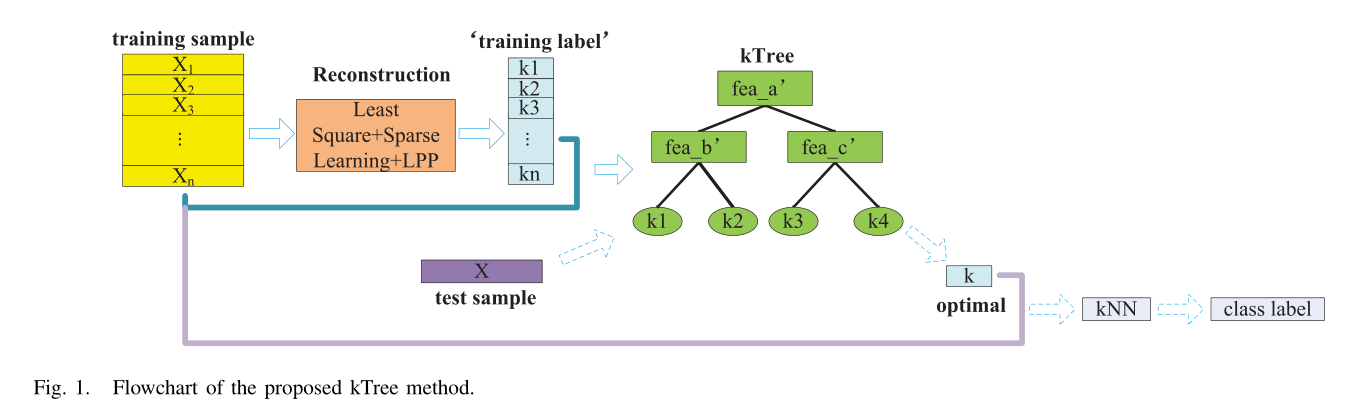
\includegraphics[scale=0.4]{kTree}

	\subsection{k*Tree方法}
	在训练阶段,在叶结点中,k*Tree除了存储最佳$ k $值,还存储定位到该叶结点的训练样本的一个子集,该子集中每个样本的k近邻,以及这些k近邻的最近邻。具体来说,每个叶结点存储一个最佳$ k $值(例如$ k_j $),训练样本的一个子集($ \mathbf{X^{'} = \lbrace {x_1^{'},...,x_m^{'}} \rbrace} $, 这些样本的最佳$ k $值为$ k_j $)。除此之外,还要存储$ \mathbf X^{'} $ 中每个样本的$ k_j $个最近邻,记为$ \mathbf{X_i^{'} = \lbrace {x_{i1}^{'},...,x_{ik_j}^{'}} \rbrace} $(其中$ i=1,2,...m $),以及每个$ x_{ik}^{'} $的最近邻,记为$ x_{ik}^{"} $。
	
	在测试阶段,给定一个测试样本,k*Tree方法首先搜索k*Tree来输出该样本的最佳$ k $值(设为$ k_t $)以及它的$ k_t $近邻。
	
	k*Tree流程图如图所示:
	
	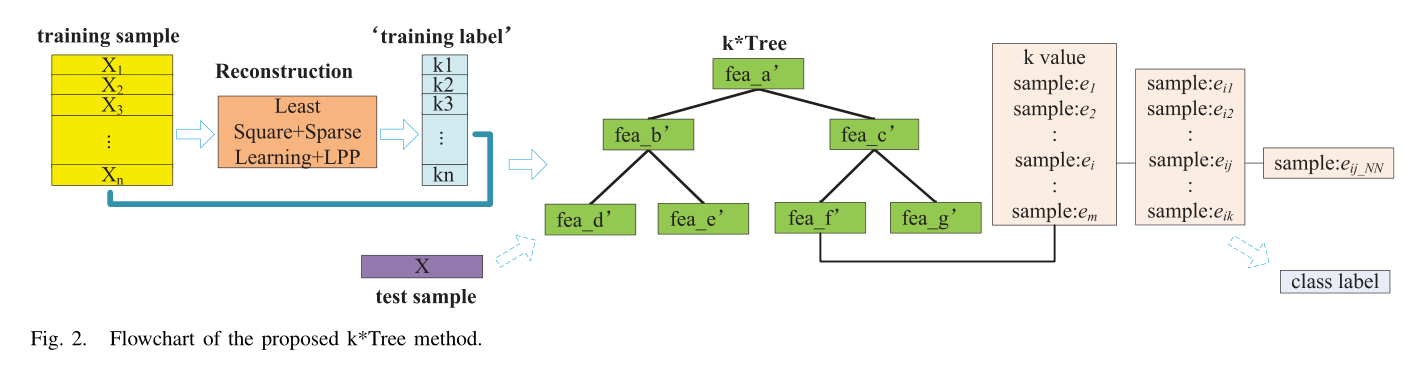
\includegraphics[scale=0.4]{kStarTree}
\end{document}